\section{Domain DSE}
\label{sec:DSE}

%This section proposes a novel domain-specific DSE for HW/SW partitioning for a domain of applications. The key insight is to broaden the scope of the exploration heuristic from a single app in isolation to a group of applications. In general, different optimization goals are possible, e.g. minimize power consumption or maximize throughput with various constraints (e.g. cost, area). In this work, we focus on throughput improvement for all applications within a certain HW budget.

In next \secref{sec:DSS} and \secref{sec:GA}, \newtext{this paper proposes two novel domain-specific DSE, DSS and GIDE,} for HW/SW partitioning for a domain of applications. The key insight is to broaden the scope of the exploration heuristic from a single app in isolation to a group of applications. In general, different optimization goals are possible, e.g. minimize power consumption or maximize throughput with various constraints (e.g. cost, area). In this work, we focus on throughput improvement for all applications within a certain HW budget.

Using the domain formalization in \secref{sec:Domain}, DSS and \ga address the problem as follows: 
\begin{problem}[DS-DSE]
	\label{p:dse}
	\normalfont{Given a domain \textit{G} and a HW budget $N$ (area), find a HW/SW partition of \textit{T} (the set of domain function types) that maximizes average throughput improvement \footnote{In DSE problem, there are multiple objectives, e.g. throughput, delay, power consumption, and area. To simplify problem and clarify result discussion, this paper only focuses on one objective throughput with the fixed area limitation (area). Multiple-objective DS-DSE problems will be in the future work.} over pure SW execution for all $\textit{g} \in \textit{G}$.}
\end{problem}


\section{Dynamic Score Selection (DSS)}
\label{sec:DSS}

This section introduces a new algorithm: dynamic score selection (DSS). It starts with a pure SW platform and then iterates through greedily selecting a composition candidate from domain features for HW realization. \newtext{Our greedy approach uses the Dynamic Composition Score (DCS: based on Domain Score) to estimate which composition is the most promising to improve domain performance considering cost.} This section, first introduces the dynamic composition score and then the DSS algorithm.


\subsection{Dynamic Composition Score (DCS)}
\label{sub:dcs}

Given the amount of applications a domain and the myriad domain platform design options, a detailed simulations or detailed analytical approaches that include scheduling effects are prohibitively expensive to execute. Instead, our approach focuses on overall processing demand (i.e. how many operations) of the domain and processing supply by the architecture (symmetric for communication). The dynamic composition score quantifies the benefits moving a composition $C$ from processor to hardware mapping. DCS estimates the benefits stemming from processing and communication mapping, scales them using dynamic weights (tuned to domain properties) and includes the additional cost of hardware implementation. 

%\vspace{-10pt}
\begingroup\makeatletter\def\f@size{9}\check@mathfonts
\begin{equation}
\begin{split}
\label{eq:scoreDSS}
	DCS &= ( B_{P} * w_{P} + B_{C} * w_{C} ) / cost\\
	cost &= \left\vert{C \cap SW}\right\vert
\end{split}
\end{equation}
\endgroup

In Eq.~\eqref{eq:scoreDSS}, $B_P$ and $B_C$ are the benefits of processing and communication if the composition is mapped on HW, respectively. \newtext{They are calculated considering both aggregated benefits and appearances, see}~\secref{sub:ben_proc} and ~\secref{sub:ben_comm}. \newtext{$w_P$ and $w_C$ are the weights to scale both benefits (}~\secref{sub:weight}). The weights are dynamically adjusted tracking performance bottlenecks, where processing or communication might be more important. Since the the DSS dynamic choosing the promising composition $C$ (multiple function types $t$) for HW implement, the consumed HW budget is need to be taken into account. The $cost$ is defined the number of additional function types (i.e. HWACCs) to realize the composition in HW. 



\subsection{DS-DSE with Dynamic Score Selection (DSS)}
\label{sub:dss}

Dynamic Score Selection (DSS) implements Domain DSE based on DCS (Sec.~\ref{sub:dcs}). Algorithm~\ref{alg:dss} illustrates the flow. DSS starts with a pure SW mapping (line 1-2) and then greedily select the best candidate for HW mapping. Candidates are all compositions (and their contained function types) of the domain (line 3). DSS evaluates their benefits using the DCS (line 5-8) given current mapping and selects highest scored candidate. With a positive score, ie. performance improvement (line9), it maps all its SW-mapped function types to HW (lines 10-12). Subsequently it updates candidates by removing HW-mapped compositions (line 13). The loop (starting at line 4) repeats until the HW budget is exhausted (line 4) or no further improvement is possible (all negative score) (line 15).

\begin{algorithm}
\caption{DSS: Dynamic Score Selection}
\label{alg:dss}
\begin{algorithmic}[1]
{\footnotesize
\State $SW \gets T$
\State $HW \gets \emptyset$
\State $Cand \gets \{C \vert C \in CS\}$
\Comment Candidates
\While{$\left\vert{HW}\right\vert < HWbudget$}
	\LineComment Processing/Communication weight calculation
	\State $(w_{P}$, $w_{C}) = weightCal(CS, SW, HW)$
	\LineComment Calculate each candidate $C$ score, return the highest
	\State $C = scoreHighest(Cand, CS, SW, HW, w_{P}, w_{C})$
	\If{$C.Score > 0$}
		\For{\textbf{each} $t \in C \cap SW$}
			\State $SW = SW \setminus \{t\}$
			\State $HW = HW \cup \{t\}$
		\EndFor
		\State $Cand = Cand \setminus \{C.t \vert C \subseteq HW \}$
	\Else
		\State Break \Comment No improvement
	\EndIf
\EndWhile
}
\end{algorithmic}
\end{algorithm}
\section{\ga}
\label{sec:GA}

Novel exploration approaches are needed that broaden the scope of DSE from single application to a domain of applications in order to design a domain-specific platforms. The enormous design space renders exhaustive search infeasible, requiring heuristics for sparse sampling. Genetic Algorithm is one of efficient heuristics algorithms with high flexibility. This section presents GenetIc Domain Exploration (\ga), a genetic algorithm with a guided local search.



%Using the domain formalization in \secref{sec:Domain}, \ga addresses the problem as follows: 
%\begin{problem}[DS-DSE]
%	\label{p:dse}
%	\normalfont{Given a domain \textit{G} and a HW budget $N$ (area), find a HW/SW partition of \textit{T} (the set of domain function types) that maximizes average throughput improvement \footnote{In DSE problem, there are multiple objectives, e.g. throughput, delay, power consumption, and area. To simplify problem and clarify result discussion, this paper only focuses on one objective throughput with the fixed area limitation (area). Multiple-objective DS-DSE problems will be in the future work.} over pure SW execution for all $\textit{g} \in \textit{G}$.}
%\end{problem}


This section introduces \ga stepwise with increasing complexity. It first introduces the baseline genetic algorithm \emph{\garand} which outlines general principles and configurations. It then extends the algorithm by \newtext{a guided local search (LS) with 3 versions} to enhance the exploration performance. 


%\vspace{4pt}
\subsection{\garand}
% overview the algorithm and introduce the main components. Each component is then described 
% in more detail in a separate paragraph. 


% reduce the white space between figure and text by 
% adjusting columnsep
% see: https://tex.stackexchange.com/questions/106144/adjusting-left-right-margins-of-a-wrapfig
	
%\begin{wrapfigure}{r}{0.5\linewidth}
%	\begin{center}
%		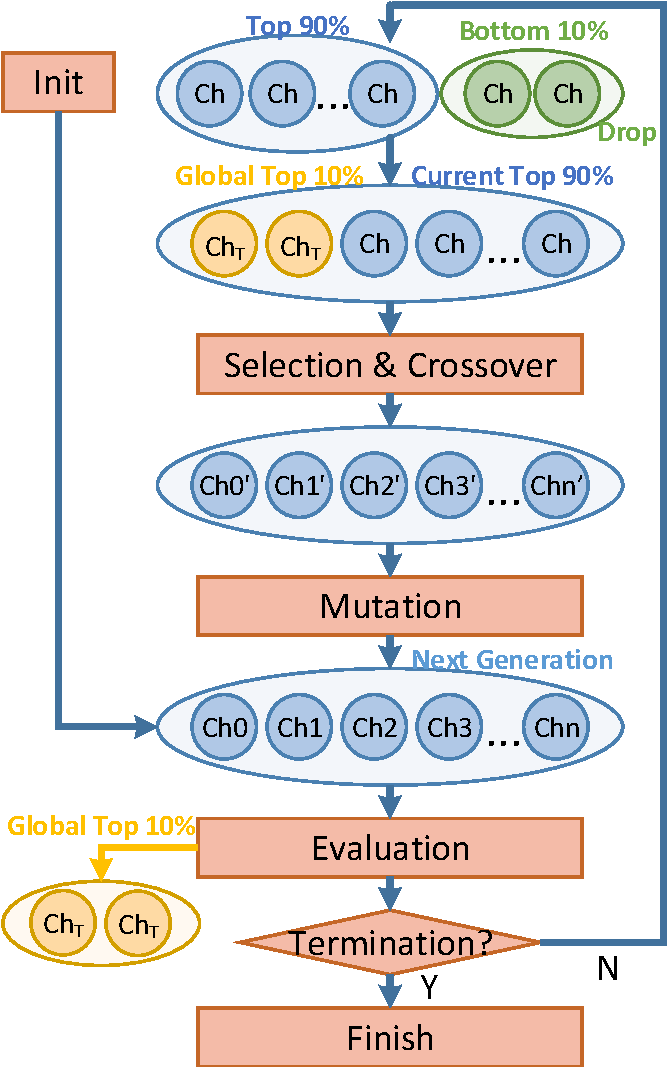
\includegraphics[width=\linewidth]{fig/pGA.pdf}
%	\end{center}
%	\vspace{-5pt}
%	\caption{Algorithm Overview}
%	\label{fig:GA}
%	%\vspace{-4pt}
%\end{wrapfigure}

\begin{figure}[h]
	\centering
	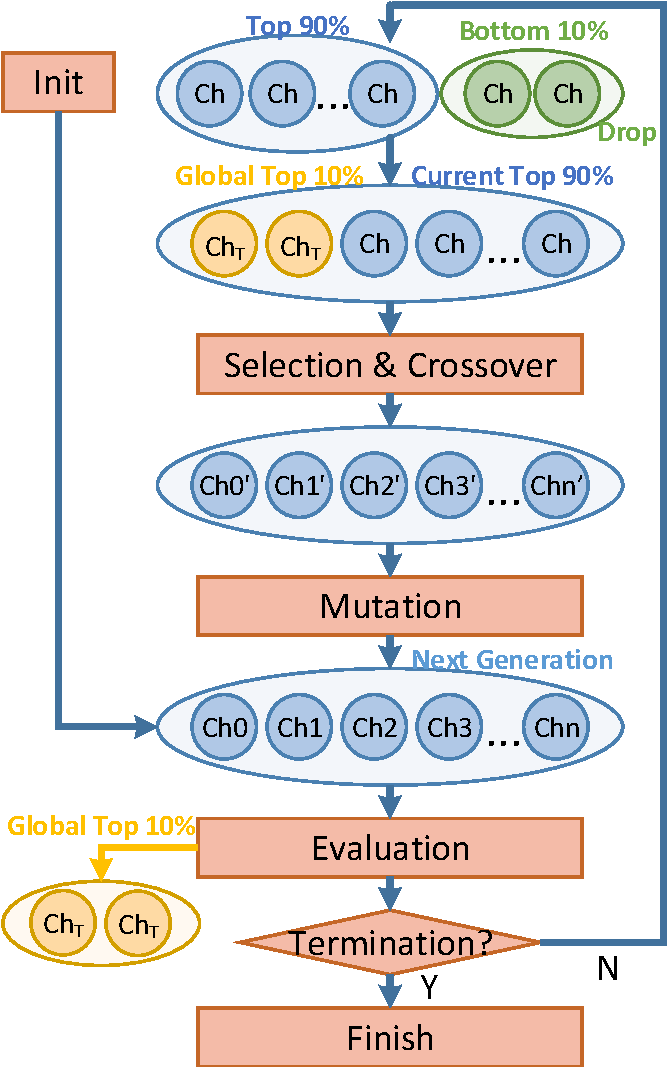
\includegraphics[width=0.5\linewidth]{fig/pGA.pdf}
	\caption{Genetic Algorithm Overview}
	\label{fig:GA}
\end{figure}

\figref{fig:GA} overviews our baseline genetic algorithm. The exploration configuration is captured in a set of \emph{chromosomes}. Each chromosome captures HW/SW mapping of each function type (FT) in the domain as a set of genes. After randomly generating an initial population, the \emph{evaluation} analyzes the fitness of each chromosome using the analytic model. The evaluation tracks global top 10\% chromosomes (across all generations). They replace the bottom 10\% in a generation to start a new population. From this, \emph{Selection \& Crossover} selects pairs of promising chromosomes swaps genes among them. To further increase variation, \emph{Mutation} randomly mutates individual genes. The resulting population is evaluated again and the process repeats until the \emph{Termination} condition is reached. The next paragraphs describe the process in detail. 



\textbf{Chromosome Definition.} An architecture is encoded as a chromosome as a string of integers, see Eq.~\eqref{eq:ch}, representing individual genes in a fixed order. Each gene ($g_A$, $g_B$ .. $g_X$) represents whether a FT ($t_{A}$,$t_{B}$ ... $t_{X}$) is implemented in SW ($g_{I} = 0$) or in HW ($g_{I} > 0$). Adding a repeated ACC with FT existed in HW has less improvement in performance, and wastes the HW budget. To simplify the large domain design space, in this paper, each FT is at most implemented once in HW. Application to platform mapping is implicit: each actor instance of a HW-implemented FT is mapped to its HW accelerator.
As outlined in \secref{sec:Platform} "Target Platform", only HW/SW communication occurs through a common system interconnect through shared memory. Consequently, connectivity, mapping to system communication fabric or memory is not encoded as they can be inferred from the HW allocation. Connectivity within the HW partition is n:n, neither needing encoding.
%
\begin{equation}
%\vspace{-6pt}
\begin{split}
\label{eq:ch}
&Ch = \{g_A, g_B, ..., g_X \}, \left\vert{Ch}\right\vert = \left\vert{T}\right\vert \\
&g_{I} = 0, t_{I} \in SW \\
&g_{I} > 0, t_{I} \in HW \\
\end{split}
\end{equation}


\textbf{Initialization.} To form the starting population, \emph{init} randomly generates chromosomes according to the defined HW budget $N$ (i.e. $\lvert HW \rvert = N$, and $\lvert SW \rvert = \lvert T \rvert - N$). The population size is dependent on the design space, which given our assumptions is mostly impacted by the number of function types $\lvert T \rvert$. Therefore, we scale the population size dependent on domain by: $\lvert P  \rvert = \lfloor 2 * \sqrt{ \lvert T \rvert} \rfloor$.

\textbf{Evaluation / Fitness Function.} Evaluating the fitness of a single chromosome requires \emph{evaluating} each domain application on the platform encoded in the chromosome, as well as \emph{aggregating} the results. Our our analytical model \secref{sec:EvaOp} computes steady state throughput for each app. To obtain a comparable quantification across apps we consider throughput improvement: scaling throughput on the candidate platform over throughput of a pure SW platform.  The \emph{aggregation} across all applications' throughput improvement determines how well the applications are represented in the domain. As we aim for an equal representation, the applications' throughput is averaged to determine the chromosome's fitness. 

To reduce the number of generations needed for a complete exploration, \ga applies an elitist bias \cite{quan2014towards}. Chromosomes are sorted by fitness. The fittest 10\% chromosomes are promoted to a global elite pool maintained across all generations. As the global elite pool is of constant size, the most elite chromosomes displace less elites. To form a new population the bottom 10\% chromosomes are dropped and replaced with the elite pool. This allows the elite genes to breed into the next generation. 

% JH very detailed question: if one generation has a chromosome propagated to the elite pool. Then this elite chromosome will be swapped back in from the elite pool. Does the SAME chromosome then exist twice in the population (once from the top 90\% of the generation and once from the elite pool)?
% JH: yes same chromosome will exist twice -> higher chance to be chosen


\textbf{Selection \& Crossover.}
From this initial pool, a weighted roulette wheel \emph{selects} chromosomes for crossover. Fitter chromosomes (using the prior evaluation results) are more likely to be selected than less fit ones. Thus, the selection prefers fitter parents with the aim to propagate the best genes, but also allows others to foster diversity. For a selected pair of parent chromosomes, the crossover stage randomly selects which genes are inherited from each parent parents (subject to the HW budget). The selection and crossover repeats until a complete new population is formed.
% cross over is for |P| times to generate |P| new chromosomes 
% HW budget exeeded: repeat selection and cross over

\textbf{Mutation.} 
After crossover, the chromosomes are subject to mutation. It randomly selects two genes with opposite state (HW/SW allocation) and inverses their state.  

%The process of crossover and mutation repeats until a population out of only new chromosomes (result of crossover and mutation) is constructed. 
% first all cross over then all mutation 

\textbf{Termination.}
Given the new population the process repeats again with evaluating the fitness of each chromosome. The GA terminates if the best solution (i.e. the fittest chromosome from the elite pool) has not improved in the last 10 generations or the maximum number of generations (100) is reached. 
% actual implementation: OpenVX and synth are with 20 fixed generatiosn
% scaling experiments stops after 10 wihtout improvment
% observed 16 generations for small, 29 for large (100 types)
% max number is theoretical (not actually implemented)


%GS disabled the stuff below as it basically repeats as intro in the next section

%While a random genetic algorithm can perform well for an application DSE, we have found that it still takes too long for domain-DSE as it relies on random mutation without guidance. To improve exploration speed, we introduce a guided local search for the mutation. The next three sections discuss alternative approaches for the guided local search. 

%Heuristic Guided Mutation

\subsection{\ga with Guided Local Search}
\label{sec:GALS}

Purely random mutation requires many generations to converge. To enhance the exploration performance, \ga employs a guided local search inspired by ~\cite{wen2011heuristic}. For each chromosome it searches for the best neighbor to propagate (instead of random mutation). The evaluation methodology for the local search is crucial for the overall exploration performance. \ga uses a hybrid approach between Domain Score (DS) and Analytic Evaluation (AE) model. In order to simplify explanation and to enable details analysis, we introduce two simpler variants first: \gads and \gaana.

%It first finds the best neighbor of a chromosome by exhaustively switching two genes with opposite states (i.e. replacing a function type for HW implementation), and then evaluates the benefit of each swap. With respect to evaluation method, we proposed three variations: (1) \gads, (2) \gaana, and (3) \gah which is the ultimate \ga implementation. 

%Instead of the random mutation implemented in GA-Random,  \emph{\gads} performs a guided local search, see \figref{fig:GADSS}, 

%We consider three variants (sorted by complexity) for guided local search: (1) a guided local search using the proposed Domain Score (\gads), (2) a guided local search using the proposed Analytical Model (\gaana) for evaluation, (3) our complete approach, \ga, which employs a hybrid DS and Analytical Model, combining their benefits.  


\subsubsection{\gads}
\label{sec:GALS-DSS}

\figref{fig:GADSS} illustrates the guided local search used instead of random mutation of \garand. \gads finds the best neighbor of a chromosome $Ch_{cur}$ by exhaustively switching two genes with opposite states, and then evaluates the benefit of each swap using \newtext{the Domain Score (DS),} see~\secref{sec:ds}.

\newtext{After finding the best neighbor}, \gads keeps the best neighbor $Ch_{BN}$ (i.e. mutation with the most benefit) over the starting chromosome $Ch_{cur}$. If the best neighbor $Ch_{BN}$ improves DS, it then becomes $Ch_{cur}$ the starting point for the next search and the process repeats. 

The search terminates if no improvement is found. The last $Ch_{BN}$ becomes one chromosome in next generation. If the first search iteration does not find any improvement, the search terminates immediately and instead of $Ch_{cur}$ a new random chromosome $Ch_{R}$ is inserted. This increases the random variation and thus the chance to escape a local optimum in the following generation(s). The local search process repeats for each chromosome $Ch0' .. Chn'$. 



\begin{figure}[h]
	\centering
	%\vspace{-10pt}
	\subfloat[GA-LS(DS),GA-LS(AE) ]{
		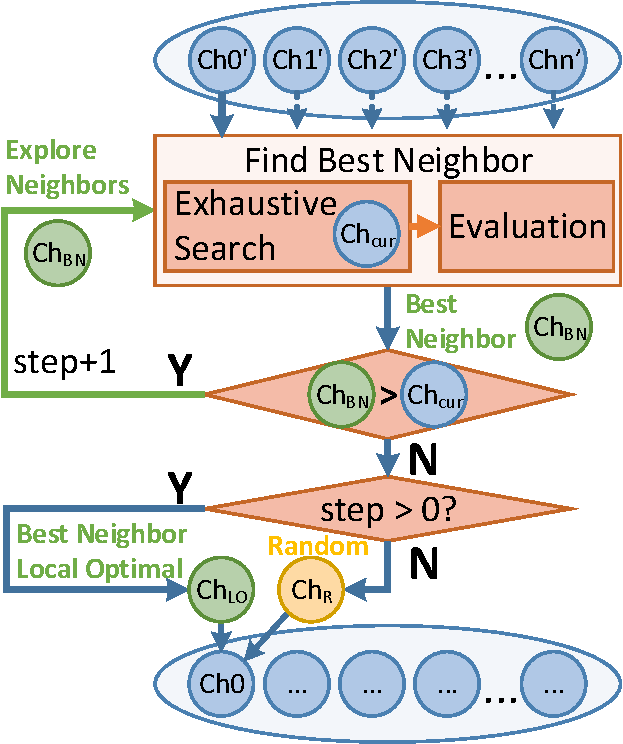
\includegraphics[width=.45\linewidth]{fig/pGADSS.pdf}
		\label{fig:GADSS}}
	\hfill
	\subfloat[GA-LS(Hybrid)]{
		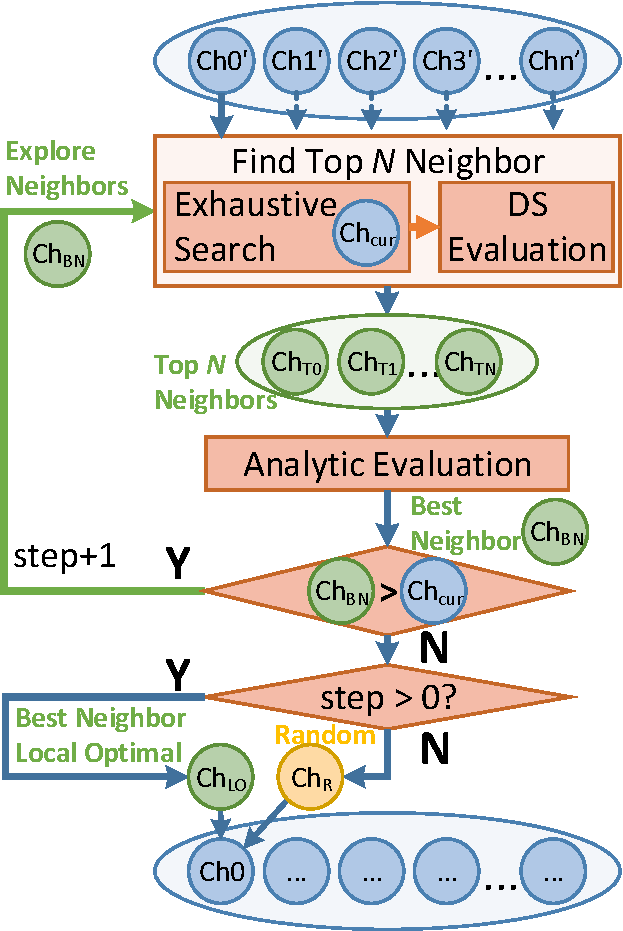
\includegraphics[width=.45\linewidth]{fig/pGADSSA.pdf}
		\label{fig:GAHybrid}}
	%\vspace{-5pt}
	\caption{Guided Local Search}
	%\vspace{-8pt}
\end{figure}

%Local search an iterative algorithm that starts with one solution, then attempts to find the best neighbor solution by exhaustive evaluate all neighbors. If the best neighbor produces a better solution compared with the original one, the best neighbor is made to the new solution, repeating until no further improvements can be found.
%In our GA algorithm, the solution is the chromosome, which defining the domain SW / HW partitioning. The neighbors of the chromosome, are (1) migrating one function type from SW(HW) to HW(SW), and (2) swap a pair of function types between SW and HW.

%Apply local search for each chromosome in generation. Using DSS to evaluate all neighbors of this chromosome, and find the best neighbors as the next step, if it has improvement. Search until no longer improvement. At the end, the mutation finds top 1 candidate (local optimal architecture) for each chromosome to form the new generation.

%If the original chromosome has been evaluated before or it is already the local optimal solution, which local search step is equal to 0, and cannot find a better neighbor in the first step of local search.
%The GA random generated a new chromosome for next generation, to help our GA to explore the large design space with more diversity.

%TODO GS Idea if the best chromosome was created just by cross over. Then, we will discard it with the approach above and replace it with a random chromosome. In effect: the absolute best solution can only be found through mutation in our setting. Improvement: after selection & chross over to a ranking by DS. Top X% of ranked chromosomes are not displaced by random, if no further improvement is found. 





\subsubsection{\gaana}

The just introduced \emph{\gads} favors speed over accuracy using the DS for evaluation in the neighborhood search. While DS is the fastest evaluation, it has limited accuracy (see \secref{sec:eva:sum}). In order to quantify the impact, we introduce the more accurate \emph{\gaana}. It realizes the same search as \emph{\gads}, however, uses the analytical model for evaluation. As the analytical model computes the performance of a single application, each application in the domain has to be evaluated and the results aggregated to determine the chromosome's fitness. This is identical to the \emph{evaluation} in \emph{\garand}. In result, the \gaana performs a very accurate local search, at the cost of exploration speed. 
\subsubsection{\gah}

In order to combine the benefits of \gads speed  and \gaana accuracy in the local search, we introduce \gah combining both approaches.

The exhaustive search over the local neighbors significantly impacts overall exploration performance. It evaluates many alternatives ($ \sum_{1 .. \lvert P \rvert} Steps_{i} * N * (\lvert T \rvert - N)$). Even considering only 1 step for each chromosome ($\lvert T \rvert$ = 50, $N$=10), already 5600 alternatives are evaluated. Hence, the fastest evaluation possible is paramount. To achieve this, \gah employs a two step approach: it first uses the faster (but less accurate) DS to identify a group of best neighbor candidates, and then re-evaluates those using the more accurate (but slower) Analytical Model to find the best neighbor. See \figref{fig:GAHybrid}. 

\gah first uses the faster evaluation \emph{DS} to find through exhaustive search the $N$ best neighbors ($Ch_{BN0}$ .. $Ch_{BNN}$) for a given chromosome $Ch_{cur}$. It then uses the analytic evaluation to select the best neighbor $Ch_{BN}$ from these candidates. The termination and random chromosome insertion are identical to \gads.

Dimensioning the group size is a local speed/accuracy trade-off. For our experiments, we opt to compare the top 5 neighbor candidates. We postulate that DS is sufficiently accurate to delineate from 400 down to 5 candidates ($\lvert T \rvert$ = 50, $N$=10). In addition, finding the absolute best in each step is not necessary as the search is iterative, improving in the next local step (or generation).


%\begin{figure}[htbp]
%	\centering
%	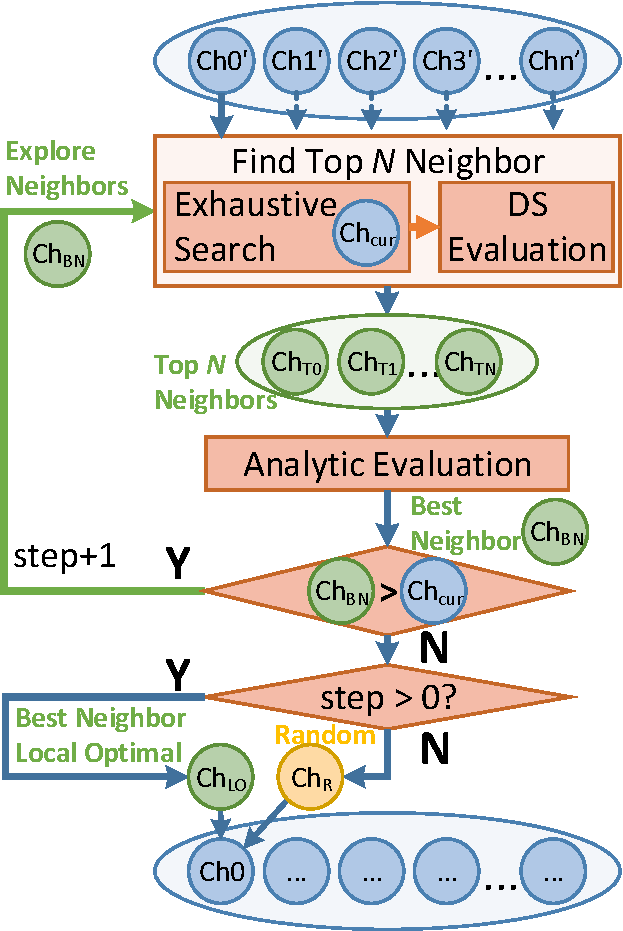
\includegraphics[width=0.48\linewidth]{fig/pGADSSA.pdf}
%	\caption{Guided Local Search (Hybrid)}
%	\label{fig:GAHybrid}
%\end{figure}



\subsection{\ga Versions Comparison}

\begin{table}[h]
	\caption{Different \ga \newtext{Comparison}}
	\label{tab:GIDE}
	\centering
	\begin{tabular}{p{0.29\linewidth}|p{0.12\linewidth}|p{0.1\linewidth}|p{0.13\linewidth}|p{0.12\linewidth}}
		\toprule
		   & GIDE-RANDOM & GIDE-DS  & GIDE-ANALYTIC & GIDE-HYBRID \\
		\hline
		\midrule
		\textbf{Local Search} & - & Y & Y & Y \\
		\hline
		\textbf{Domain Score guided} & - & Y & - & Y \\
		\hline
		\textbf{Analytic Eval guided} & - & - & Y & Y \\
		\bottomrule
	\end{tabular}
\end{table}

\tabref{tab:GIDE} \newtext{summaries the different versions of GIDE described in previous sections.} \garand \newtext{is normal genetic algorithm  without guided local search in mutation.} \gads and \gaana \newtext{are genetic algorithms with one level guided local search.} \gads \newtext{uses the Domain Score (DS) to guide local search, which has high speed but low accuracy of estimation.} While \gaana \newtext{has slow but high accurate guided local search, using Analytic Evaluation (AE).} \gah \newtext{has two-level guided, combining DS and AE, which balance the speed and accuracy.}  



 %The heuristics methods are comprised of an algorithm to explore design space and a fast evaluation/estimation to judge the performance/benefit of each iteration/selection.

%Given the very large design space, methods for efficiently traversing the design space, such as genetic algorithms \cite{abdeen2014multi}, simulated annealing \cite{liang2013hardware}, tabu search \cite{wu2013efficient}, and greedy algorithms \cite{tang2015hardware}, are important. 

% need to describe the problem.
% see also end of 3.2 



